%===================================================================
% PHẦN NÀY DO: Nguyễn Khánh Linh phụ trách
% Nội dung: Client-Side Caching (Frame Buffer) + Pre-buffer N frames
%===================================================================

\section{Client-Side Caching và Pre-buffering}

\subsection{Mục tiêu và vấn đề cần giải quyết}
Trong truyền video bằng RTP/UDP, các gói tin được gửi liên tục nhưng \textbf{không đảm bảo đến đều theo thời gian}. Nguyên nhân là do \textit{network jitter} — tức là \textbf{sự dao động độ trễ} của các gói khi đi qua mạng. Nói đơn giản, có gói đến sớm hơn dự kiến, có gói đến muộn hơn dự kiến, làm cho \textbf{khoảng thời gian giữa các lần nhận packet không ổn định}. Jitter thường xuất hiện do hiện tượng xếp hàng tại router/switch (queueing), tải mạng thay đổi, hoặc môi trường Wi-Fi nhiễu.

Nếu client \textbf{hiển thị frame ngay khi nhận được} (nhận đến đâu phát đến đó), thì chỉ cần một số gói đến muộn hoặc đến không đều sẽ dẫn đến:
\begin{itemize}
    \item Video bị \textbf{giật/khựng (stuttering)} vì thiếu frame đúng thời điểm cần phát.
    \item \textbf{FPS không đều}: lúc thì frame đến dồn dập, lúc thì bị trễ, khiến tốc độ phát không ổn định.
    \item Khi gặp trễ kéo dài ngắn hạn (burst delay), client có thể \textbf{bị đứng hình} do không còn dữ liệu để phát.
\end{itemize}

\textbf{Mục tiêu:} triển khai \textbf{client-side caching} bằng bộ đệm khung hình và \textbf{pre-buffer N frames} để hấp thụ jitter ngắn hạn, giúp video phát mượt hơn và duy trì FPS ổn định gần với FPS mục tiêu (TARGET_FPS = 50).


\subsection{Ý tưởng giải pháp}
Giải pháp của nhóm tập trung đúng vào hai yêu cầu chính của bài: \textbf{client-side caching} và \textbf{pre-buffer N frames}. Thay vì hiển thị (render) ngay lập tức khi nhận được dữ liệu từ mạng, client sẽ đệm dữ liệu vào bộ nhớ tạm để triệt tiêu ảnh hưởng của jitter và đảm bảo tốc độ phát ổn định.

\begin{itemize}
    \item \textbf{Client-Side Caching:} Client \textbf{không phát ngay} khi vừa nhận được các gói RTP. Thay vào đó, client sẽ \textbf{chờ ghép đủ dữ liệu thành một frame hoàn chỉnh}. Khi frame hoàn tất (nhận biết bằng \texttt{marker=1}), client gom dữ liệu của frame lại và lưu vào \texttt{frame buffer} (kèm vài thông tin như số frame, timestamp, kích thước,\ldots). 
    Nhờ cách này, việc \textbf{nhận dữ liệu từ mạng} và việc \textbf{hiển thị video} được tách riêng: mạng có thể lúc nhanh lúc chậm, nhưng video vẫn có thể phát ổn định hơn vì đã có buffer ``đỡ'' ở giữa.

    \item \textbf{Pre-buffer N frames:} Trước khi bắt đầu phát, client cần \textbf{tích lũy trước ít nhất N frame} trong \texttt{frame buffer} (tham số \texttt{buffer\_target = 50}). 
    Nếu số frame trong buffer còn nhỏ hơn $N$ thì client ở trạng thái \textit{BUFFERING} và tiếp tục chờ nhận thêm dữ liệu. Khi buffer đã đủ ($|Q|\ge N$), client chuyển sang \textit{PLAYING} và bắt đầu lấy frame ra phát đều theo FPS mục tiêu. 
    Cơ chế này giúp giảm hiện tượng \textbf{giật/khựng ở những giây đầu}, và nếu đang phát mà buffer bị cạn (underrun) thì client có thể \textbf{tạm dừng để nạp lại} rồi phát tiếp thay vì đứng hình liên tục.
\end{itemize}



\newpage
\subsection{Kiến trúc Producer--Buffer--Consumer}
Để chống jitter hiệu quả, hệ thống không xử lý ``nhận đến đâu phát đến đó'' nữa, mà tách rõ thành \textbf{2 luồng chạy song song} và một \textbf{vùng đệm ở giữa}. Có thể hiểu đơn giản: một luồng \textit{chuyên đi lấy dữ liệu về}, một luồng \textit{chuyên phát video}, còn bộ đệm đóng vai trò như ``kho chứa tạm'' để làm cho việc phát ổn định hơn.
\begin{itemize}
    \item \textbf{Reception thread (Producer):} Luồng này luôn lắng nghe trên socket RTP để nhận các gói tin từ server. Do một frame có thể bị chia thành nhiều gói nhỏ (fragment), reception thread sẽ \textbf{ghép các mảnh lại} cho đến khi tạo thành \textbf{một frame hoàn chỉnh}. Khi ghép xong, luồng này \textbf{không hiển thị ngay} mà sẽ đưa frame vào bộ đệm. Có thể xem đây là ``người sản xuất'' liên tục tạo ra frame và nạp vào kho.
    \item \textbf{Frame Buffer (Deque):} Đây là \textbf{hàng đợi các frame hoàn chỉnh} nằm giữa 2 luồng. Buffer dùng cấu trúc \texttt{deque} vì thêm vào cuối và lấy ra đầu đều nhanh. Buffer được đặt \textbf{giới hạn dung lượng} (\texttt{maxlen = 200}) để tránh trường hợp mạng quá nhanh hoặc phát quá chậm làm bộ nhớ tăng mãi và gây tràn RAM. Nói đơn giản, buffer giống như một ``bình chứa'' để giữ sẵn một lượng frame dự phòng, giúp video không bị giật khi mạng chập chờn trong thời gian ngắn.
    \item \textbf{Playback thread (Consumer):} Luồng này chịu trách nhiệm \textbf{lấy frame từ buffer ra phát} theo nhịp cố định (FPS mục tiêu). Nghĩa là dù mạng nhận lúc nhanh lúc chậm, playback thread vẫn cố gắng hiển thị đều đặn để tạo cảm giác mượt. Nếu buffer còn đủ frame thì video chạy ổn định; nếu buffer cạn (underrun) thì playback thread sẽ tạm chờ để buffer được nạp lại rồi phát tiếp. Có thể xem đây là ``người tiêu thụ'' lấy hàng từ kho ra sử dụng.
\end{itemize}
Nhờ kiến trúc này, việc \textbf{nhận dữ liệu theo nhịp mạng} và việc \textbf{phát video theo nhịp FPS} được tách rời, nên jitter sẽ ít ảnh hưởng trực tiếp đến trải nghiệm xem video.


% Preamble:
% \usepackage{tikz}
% \usetikzlibrary{positioning,arrows.meta}

\begin{figure}[H]
\centering
\begin{tikzpicture}[
    node distance=1.2cm,
    box/.style={draw, rounded corners, minimum width=6cm, minimum height=0.95cm, align=center},
    arrow/.style={-{Stealth[length=3mm,width=2mm]}, thick}
]
    \node[box] (rtp) {RTP Packets};
    \node[box, below=of rtp] (recv) {Reception Thread\\(Producer)};
    \node[box, below=of recv] (buf) {Frame Buffer (deque)\\Bounded Queue};
    \node[box, below=of buf] (play) {Playback Thread\\(Consumer)};
    \node[box, below=of play] (disp) {Display / GUI};

    \draw[arrow] (rtp) -- (recv);
    \draw[arrow] (recv) -- (buf);
    \draw[arrow] (buf) -- (play);
    \draw[arrow] (play) -- (disp);

    % Optional side notes (em có thể xóa nếu muốn gọn)
    \node[right=0.6cm of recv, align=left] (note1) {\footnotesize Receive \& reassemble\\\footnotesize (marker=1)};
    \node[right=0.6cm of buf, align=left] (note2) {\footnotesize Pre-buffer $N$ frames\\\footnotesize Absorb jitter};
    \node[right=0.6cm of play, align=left] (note3) {\footnotesize Pop at fixed FPS\\\footnotesize handle underrun};

    \draw[-, thin] (note1.west) -- ++(-0.3,0);
    \draw[-, thin] (note2.west) -- ++(-0.3,0);
    \draw[-, thin] (note3.west) -- ++(-0.3,0);
\end{tikzpicture}
\caption{Mô hình Producer--Buffer--Consumer chống jitter}
\label{fig:producer-buffer-consumer}
\end{figure}


\subsection{Thiết kế bộ đệm và tham số điều khiển}
\begin{itemize}
    \item \textbf{Buffer capacity} (\texttt{maxlen=200}): bộ đệm được cài đặt bằng \texttt{deque} với \texttt{maxlen=200}, nghĩa là tối đa chỉ lưu \textbf{200 frame} trong RAM. Đây là \textit{bounded buffer} để tránh việc buffer phình to vô hạn khi mạng gửi nhanh hoặc client phát chậm, từ đó giảm nguy cơ \textbf{OOM (Out Of Memory)} — tình trạng chương trình bị \textit{hết bộ nhớ RAM} và có thể bị treo hoặc bị hệ điều hành buộc đóng.
    \item \textbf{Pre-buffer threshold} ($N = \texttt{buffer\_target} = 50$): ngưỡng \textbf{số frame tối thiểu} mà client phải tích lũy trong \texttt{frame\_buffer} trước khi cho phép bắt đầu phát video. Cụ thể, nếu $|Q| < N$ (buffer chưa đủ 50 frame) thì client vẫn ở trạng thái \textit{BUFFERING} và tiếp tục nhận dữ liệu để làm đầy bộ đệm; chỉ khi $|Q|\ge 50$ thì client mới chuyển sang \textit{PLAYING} và playback thread bắt đầu \texttt{popleft()} frame để hiển thị theo FPS mục tiêu. Với \texttt{TARGET\_FPS = 50}, ngưỡng $N=50$ tương đương khoảng $50/50 \approx 1$ giây dữ liệu video được đệm sẵn trước khi phát, giúp giảm hiện tượng giật/khựng ở thời điểm bắt đầu.
    \item \textbf{Playback rate (FPS):} tốc độ phát \textbf{mục tiêu} mà client cố gắng duy trì khi hiển thị video. Trong code, nhóm đặt \texttt{TARGET\_FPS = 50} nên mỗi frame có thời lượng mong muốn là
    \[\texttt{FRAME\_DURATION} = \frac{1}{\texttt{TARGET\_FPS}} = \frac{1}{50} \approx 0.02 \text{ giây/frame}.\]Ở mỗi vòng lặp phát, chương trình đo thời gian xử lý thực tế của frame (giải mã, ghi file tạm, cập nhật GUI,\ldots) rồi \textbf{sleep phần thời gian còn lại}:\[\texttt{sleep\_time} = \max(0, \texttt{FRAME\_DURATION} - \texttt{elapsed}),\]nhờ đó playback thread phát frame theo nhịp đều đặn gần 50 FPS (nếu buffer còn đủ dữ liệu). Nếu xử lý một frame mất lâu hơn \texttt{FRAME\_DURATION} thì \texttt{sleep\_time} sẽ bằng 0 và FPS thực tế sẽ giảm xuống tương ứng.
    \item \textbf{Timeout end-of-stream} ($T_{end}$): cơ chế phát hiện \textbf{hết video} khi đang phát mà \texttt{frame\_buffer} bị rỗng quá lâu. Trong \texttt{playFromBuffer()}, mỗi lần buffer rỗng chương trình sẽ tăng biến đếm \texttt{empty\_buffer\_count} và chờ thêm \texttt{0.1s}. Nếu tình trạng rỗng kéo dài vượt ngưỡng, client kết luận \textbf{end-of-stream} (server đã gửi hết dữ liệu hoặc không còn gói đến), cập nhật trạng thái ``Video ended'' và dừng playback thread.
    Với cấu hình hiện tại, điều kiện là:
    \[
    \texttt{empty\_buffer\_count} > 50 \;\;\Rightarrow\;\; T_{end} \approx 50 \times 0.1 = 5 \text{ giây}.
    \]
    Nghĩa là nếu trong khoảng $\sim 5$ giây liên tục không lấy được frame nào từ buffer, client sẽ xem video đã kết thúc.

\end{itemize}

\subsection{Các trạng thái của bộ đệm}
\begin{table}[H]
\centering
\begin{tabular}{|l|l|l|}
\hline
\textbf{Trạng thái} & \textbf{Điều kiện} & \textbf{Hành động} \\ \hline
BUFFERING & $|Q| < N$ & Chờ nhận thêm frame (pre-buffer) \\ \hline
PLAYING & $|Q| \ge N$ & Pop và phát theo FPS cố định \\ \hline
UNDERRUN & $|Q|=0$ khi đang PLAYING & Tạm dừng phát, quay lại BUFFERING \\ \hline
END & $|Q|=0$ quá $T_{end}$ & Dừng playback, báo kết thúc \\ \hline
\end{tabular}
\caption{Các trạng thái của bộ đệm}
\end{table}

\subsection{Thuật toán}
\subsubsection{Thuật toán Reception (Producer) trong \texttt{listenRtp()}}
\begin{enumerate}
    \item Nhận một gói RTP từ socket, giải mã các trường: \texttt{seqNum}, \texttt{timestamp}, \texttt{marker}, \texttt{payload}.
    \item Gọi \texttt{network\_analyzer.record\_packet(...)} để ghi nhận thống kê mạng.
    \item Nếu đây là gói đầu tiên của một frame mới (\texttt{current\_frame\_ts} chưa được gán), khởi tạo trạng thái ghép frame:
    đặt \texttt{current\_frame\_ts = timestamp}, \texttt{frame\_corrupted = False}, đồng thời đặt
    \texttt{expected\_seq = seqNum + 1} (vì gói hiện tại đã được xử lý).
    \item Nếu \texttt{timestamp} khác \texttt{current\_frame\_ts}:
    \begin{itemize}
        \item Nếu \texttt{timestamp} nhỏ hơn \texttt{current\_frame\_ts} (gói đến trễ của frame cũ) thì bỏ qua gói này.
        \item Nếu \texttt{timestamp} lớn hơn \texttt{current\_frame\_ts} trong khi đang ghép dở frame hiện tại (chưa kết thúc), coi frame hiện tại không còn hợp lệ và reset để bắt đầu ghép frame mới.
    \end{itemize}
    \item Kiểm tra thứ tự theo \texttt{expected\_seq}:
    \begin{itemize}
        \item Nếu \texttt{seqNum == expected\_seq}: nối \texttt{payload} vào vùng ghép frame và tăng \texttt{expected\_seq} lên 1.
        \item Nếu \texttt{seqNum > expected\_seq}: phát hiện có mất gói (gap) trong frame $\Rightarrow$
        đặt \texttt{frame\_corrupted = True}, vẫn nối \texttt{payload} hiện tại và cập nhật \texttt{expected\_seq = seqNum + 1}.
        \item Nếu \texttt{seqNum < expected\_seq}: gói đến trễ / out-of-order / duplicate $\Rightarrow$ bỏ qua để tránh ghép sai thứ tự.
    \end{itemize}
    \item Khi \texttt{marker=1} (kết thúc frame):
    \begin{itemize}
        \item Nếu \texttt{frame\_corrupted=True} thì loại bỏ frame này (tránh lỗi JPEG bị hỏng/truncated) và reset trạng thái ghép frame.
        \item Nếu frame hợp lệ thì đóng gói thành \texttt{frame\_info} và đưa vào \texttt{frame\_buffer} (deque) dưới khóa \texttt{buffer\_lock}, sau đó reset trạng thái để ghép frame kế tiếp.
    \end{itemize}
\end{enumerate}



\subsubsection{Thuật toán Playback + Pre-buffer (Consumer)}
\begin{enumerate}
    \item Nếu $|Q| < N$: hiển thị trạng thái BUFFERING và chờ (pre-buffer).
    \item Nếu $|Q| \ge N$: lấy 1 frame từ đầu hàng đợi (\texttt{popleft}) và hiển thị.
    \item Điều chỉnh thời gian ngủ để giữ FPS ổn định.
    \item Nếu $|Q|=0$ khi đang PLAYING: chuyển UNDERRUN và quay lại BUFFERING.
    \item Nếu buffer rỗng quá $T_{end}$: kết luận END và dừng phát.
\end{enumerate}

\subsection{Minh họa ngắn bằng code}
\begin{lstlisting}[language=Python, caption={Khởi tạo buffer và đồng bộ truy cập}]
from collections import deque
import threading

self.frame_buffer = deque(maxlen=200)   # bounded buffer
self.buffer_target = 50                 # pre-buffer N frames
self.buffer_lock = threading.Lock()     # thread-safe
\end{lstlisting}

\begin{lstlisting}[language=Python, caption={Nguyên tắc producer/consumer}]
# Producer: khi frame hoan thanh
with self.buffer_lock:
    self.frame_buffer.append(frame_info)

# Consumer: khi du buffer_target
with self.buffer_lock:
    frame_info = self.frame_buffer.popleft()
\end{lstlisting}


\subsection{Đánh đổi (Trade-off) và kết quả kỳ vọng}
Để đánh giá hiệu quả của cơ chế client-side caching và pre-buffering,
nhóm tiến hành chạy thử nghiệm với video HD \texttt{sample\_1920x1080.mjpeg}.
Server thực hiện pre-buffer 60 frames trước khi phát và đo các chỉ số
hiệu năng trong quá trình streaming.

\begin{table}[H]
\centering
\renewcommand{\arraystretch}{1.2}
\begin{tabular}{|l|c|}
\hline
\textbf{Chỉ số (Client)} & \textbf{Giá trị đo được} \\ \hline
Frame rate trung bình & 48.1 FPS \\ \hline
Bandwidth trung bình & 27.75 Mbps \\ \hline
Packet loss & 0.0\% (0 packets) \\ \hline
Network jitter & 2.88 ms \\ \hline
Frames nhận được & 319 frames \\ \hline
Dung lượng video nhận & 31.6 MB \\ \hline
Quality level & ULTRA (MTU = 1450) \\ \hline
\end{tabular}
\caption{Số liệu thực nghiệm phía Client thu thập từ GUI}
\label{tab:client-gui-stats}
\end{table}

Hình~\ref{fig:client-gui} minh họa trực quan các chỉ số thống kê phía client
trong quá trình streaming, được dùng để thu thập số liệu ở Bảng~\ref{tab:client-gui-stats}.

\begin{figure}[H]
    \centering
    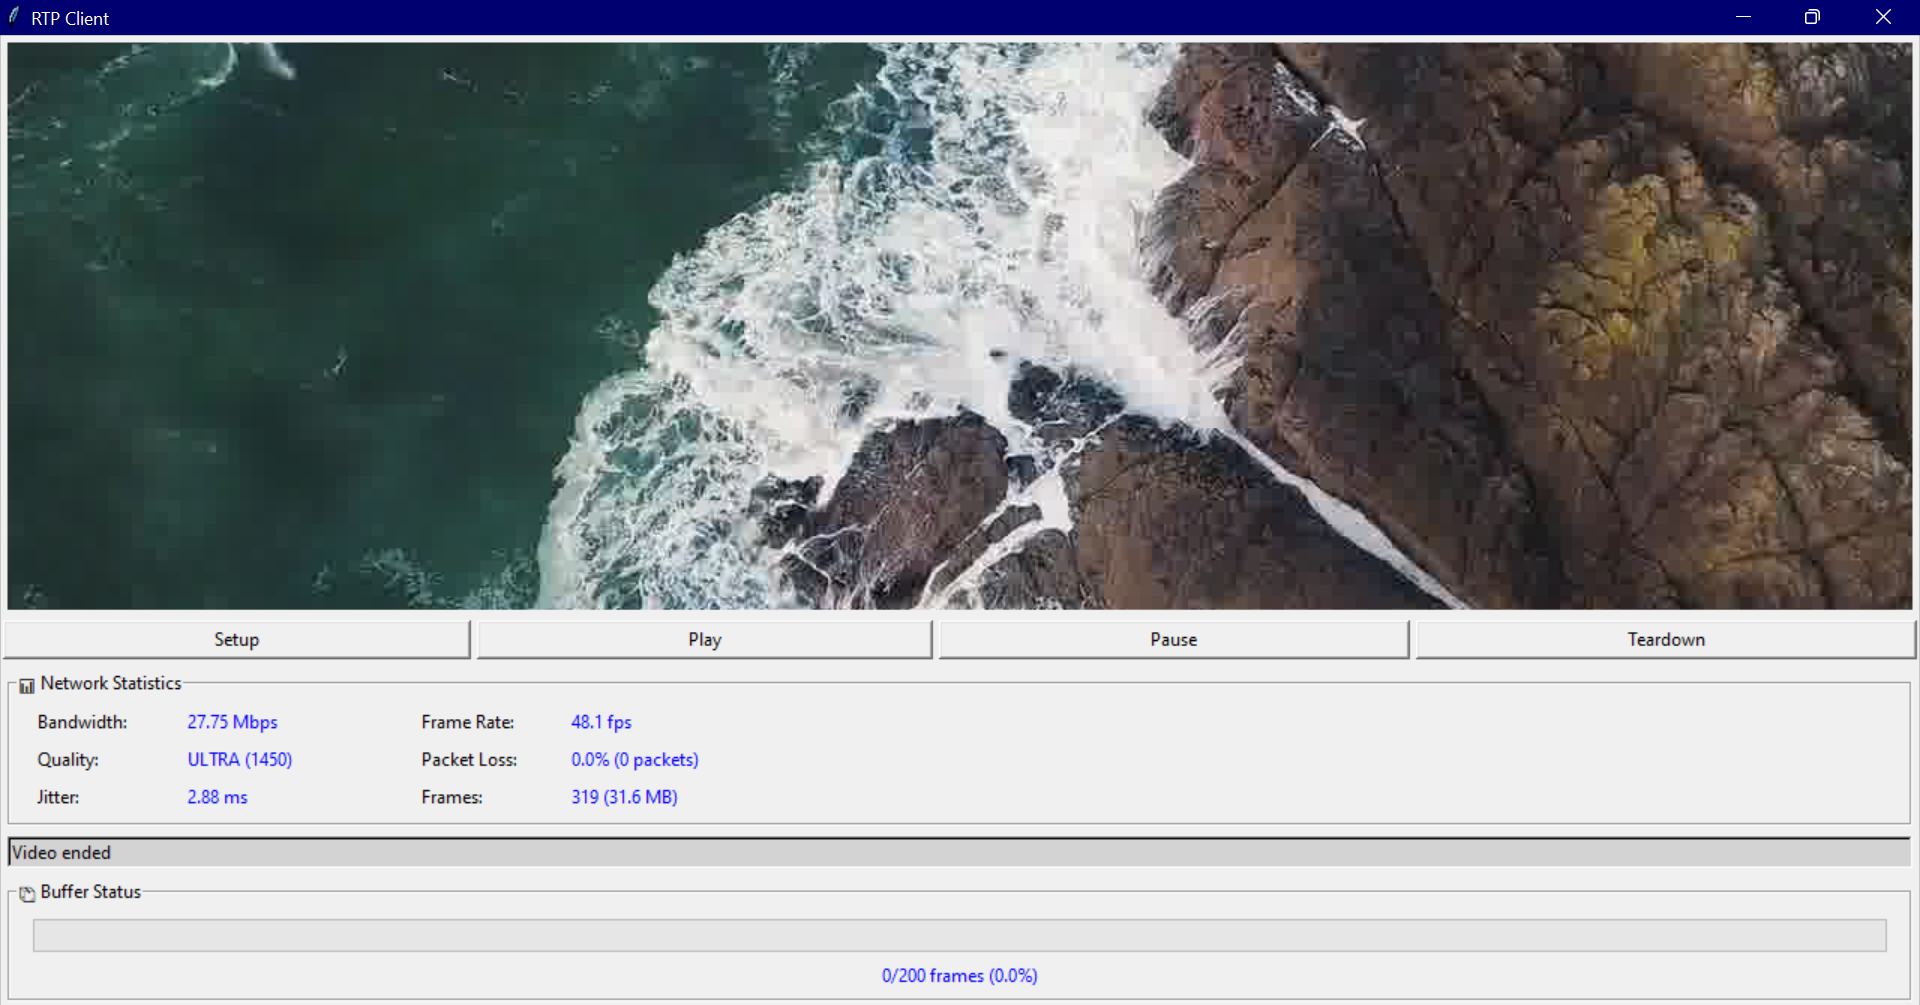
\includegraphics[width=0.95\textwidth]{GUI.png}
    \caption{Giao diện chương trình Client với thống kê mạng và trạng thái buffer}
    \label{fig:client-gui}
\end{figure}



\begin{itemize}
    \item \textbf{Đánh đổi (Trade-off):} cơ chế pre-buffer làm tăng độ trễ ban đầu trước khi phát video vì client cần tích lũy đủ $N$ frame trong bộ đệm. Độ trễ này xấp xỉ $\frac{N}{FPS}$ giây. Với cấu hình đang sử dụng ($N=50$, $FPS=50$), thời gian chờ khởi động (startup delay) vào khoảng $1$ giây. Đây là đánh đổi chấp nhận được để đổi lấy trải nghiệm phát ổn định hơn.
    
    \item \textbf{Lợi ích đạt được:} việc tách riêng hai luồng \textit{reception} và \textit{playback} theo mô hình producer--consumer giúp client không phụ thuộc trực tiếp vào nhịp đến không đều của các gói RTP. Khi jitter tăng hoặc có các đợt trễ ngắn hạn, bộ đệm vẫn cung cấp frame liên tục cho playback thread, nhờ đó giảm hiện tượng giật (stuttering), hạn chế tụt FPS tức thời và giữ tốc độ phát gần với FPS mục tiêu.
    
    \item \textbf{Kết quả thực nghiệm:} số liệu ghi nhận cho thấy phía server duy trì hiệu năng streaming tương đối ổn định với trung bình $46.9$ FPS và bitrate khoảng $37.48$ Mbps, đủ để cấp dữ liệu cho phía client. Ở phía client (thông qua thống kê trên GUI), jitter trung bình khoảng $2.88$ ms, frame rate đạt $48.1$ FPS (gần sát mức mục tiêu 50 FPS) và packet loss $0.0\%$. FPS client là FPS hiển thị đo trên GUI (playback rate), còn FPS server là FPS gửi. Hai cách đo khác nhau nên có thể lệch nhẹ.” Các kết quả này cho thấy cơ chế client-side caching kết hợp pre-buffering đã hoạt động hiệu quả: playback ổn định hơn, giảm ảnh hưởng của biến động mạng và cải thiện chất lượng trải nghiệm trong suốt quá trình xem video. 
\end{itemize}

\subsection{Kết luận}
Nhóm triển khai client-side caching bằng bộ đệm khung hình (deque) và cơ chế pre-buffer N frames.
Thiết kế tách reception/playback theo mô hình producer--consumer giúp hấp thụ jitter và giữ FPS ổn định trong quá trình phát.

\newpage